%\linenumbers*
\chapter{EFFECT OF WITHIN-STORM RAINFALL INTENSITY PATTERN ON SOIL EROSION}
\label{sec:EFFECTSOFRAINFALLINTENSITYCHANGESONSOILEROSION}

\section{Introduction}
\label{sec:IntensiyPatternsIntroduction}

In the last two chapters, the effect of temporal resolutions and WSGs on
soil erosion have been investigated.
In Chapter \ref{sec:EFFECTSOFTEMPORALSCALESOFSTROMDATA}, first of all, it was
shown that time-to-peak intensity ($t_p$) was affected by temporal resolution
of rainfall data. When time-to-peak intensity changes, overall shape of
rainfall storm, which can be termed as Within-Storm Intensity Pattern (WSIP),
changes together. For example, when a peak intensity occurs at the later stage
of a storm, WSIP becomes a skewed triangular shape towards the end of rainfall
duration (cf. Figure \ref{fig:weppinputincrease2hr}). As suggested previously,
time-to-peak may have an impact on erosion estimations. Thus, WSIP may too
have impacts on runoff initiation as well as soil loss amount.

Secondly, in Chapter \ref{sec:EFFECTSOFCONTINOUSANDDISCONTINUSSTORM}, it was
pointed out that WEPP changed WSIVs when modified the original rainfall
intensity information. WSIVs are closely related to WSIP. For example, when
``rainfall intensity'' within a storm increases steadily from low to high (i.e.\
increasing intensity), WSIP becomes a skewed triangular shape towards the end of
rainfall duration (cf. Figure \ref{fig:weppinputincrease2hr}). The same
principle applies to decreasing or constant, or more complex shapes. In
addition, the change of WSIP may occur when WSGs are removed from
original rainfall data as previously illustrated in Figure
\ref{fig:rainfall_discont_cont}.

Therefore, this chapter investigates the effect of rainfall intensity changes
(i.e.\ WSIVs) within storm duration in terms of WSIP by using WEPP, EUROSEM and
RillGrow.
In reality, rainfall intensity is constantly changing throughout the storm
period. It may increase or decrease and changes in more complex ways. For the
modelling purpose, however, design storms are used in this chapter. This is
because design storms are easier to compare each other without any additional
data preparation. Also, by using design storms, it is easier to separate out
a factor that is in interest without changing other factors.


\section{Simulation Data and Methods}
\label{sec:IntensiyPatternsMethods}

Rainfall storms with varying WSIP---increasing, decreasing,
increasing-decreasing and constant---are constructed as CLIGEN data by changing
time-to-peak ($t_p$) values. The constant WSIP are achieved by setting both
$t_p$ and $i_p$ to 1.0. Amounts of these rainfalls are also kept the same. In
order to investigate only effects of WSIP changes on erosion estimation. Only
one peak intensity (or no peak for the constant intensity) per storm is assumed
for model simulations because of WEPP requirements.

Two designed storms with average intensity of 10 mm/hr (120 mm for 12 hr, Figure
\ref{fig:weppeurosemintensityinputstwelvehours})
and 60 mm/hr (120 mm for 2 hr, Figure
\ref{fig:weppeurosemintensityinputstwohours}) are prepared for WEPP and EUROSEM
simulations . Two different intensities are used here in order to investigate
effects of WSIP changes in storms with low and high rainfall intensities.
Intensity of 10 mm/hr is selected because it is approximately
the same as the average intensity (12.8 mm/hr) of the rainfall storm that occurs
in the study area, South Downs, UK (see page \pageref{sec:EventRainfallData},
Chapter \ref{sec:SIMULATIONDATAMODELSANDMETHODS}). Also, the higher intensity
(i.e.\ 60 mm/hr) is selected because it is approximately the same level as the
average maximum intensity (63 mm/hr) in the study area (see page
\pageref{sec:EventRainfallData}, Chapter
\ref{sec:SIMULATIONDATAMODELSANDMETHODS}).

Firstly, for WEPP simulations, these two rainfall data are used as CLIGEN data
format. Then, as described previously in Chapter
\ref{sec:EFFECTSOFTEMPORALSCALESOFSTROMDATA} (see Figure
\ref{fig:eurosem_cligen_workaround}, page
\pageref{fig:eurosem_cligen_workaround}), WEPP-disaggregated breakpoint data for
the same rainfall storms are used for EUROSEM simulations. This enables the use
of the same data sets for WEPP and EUROSEM simulations.

\begin{figure}[htbp]
  \centering
  \subfloat[]{%
  \label{fig:weppinputincrease6hr}
  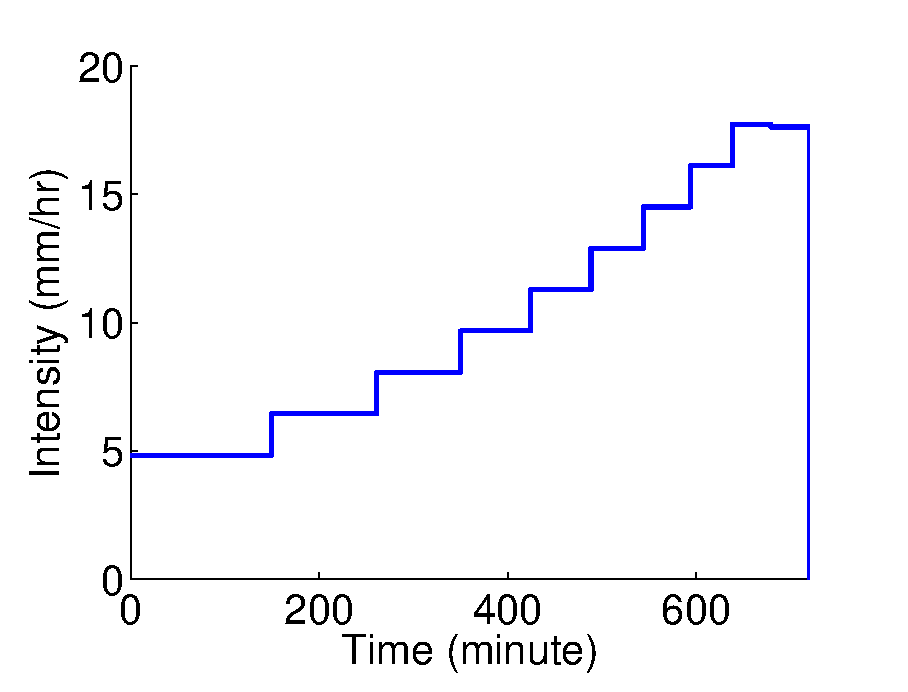
\includegraphics[width=0.24\textwidth]{./img/wepp_input_increase_6hr}}
  \subfloat[]{%
  \label{fig:weppinputdecrease6hr}
  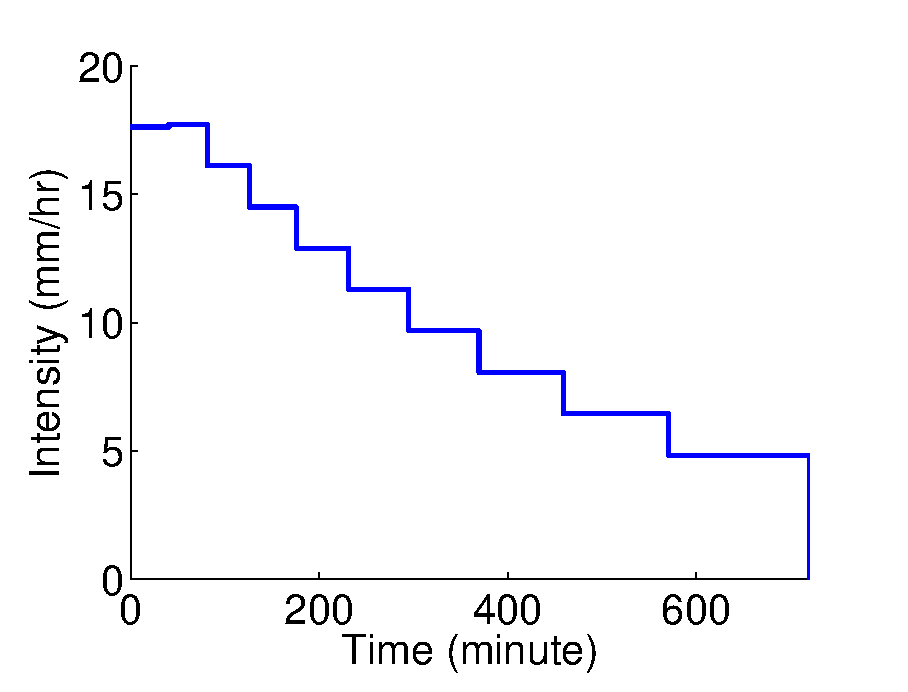
\includegraphics[width=0.24\textwidth]{./img/wepp_input_decrease_6hr}}
  \subfloat[]{%
  \label{fig:weppinputcontrol6hr}
  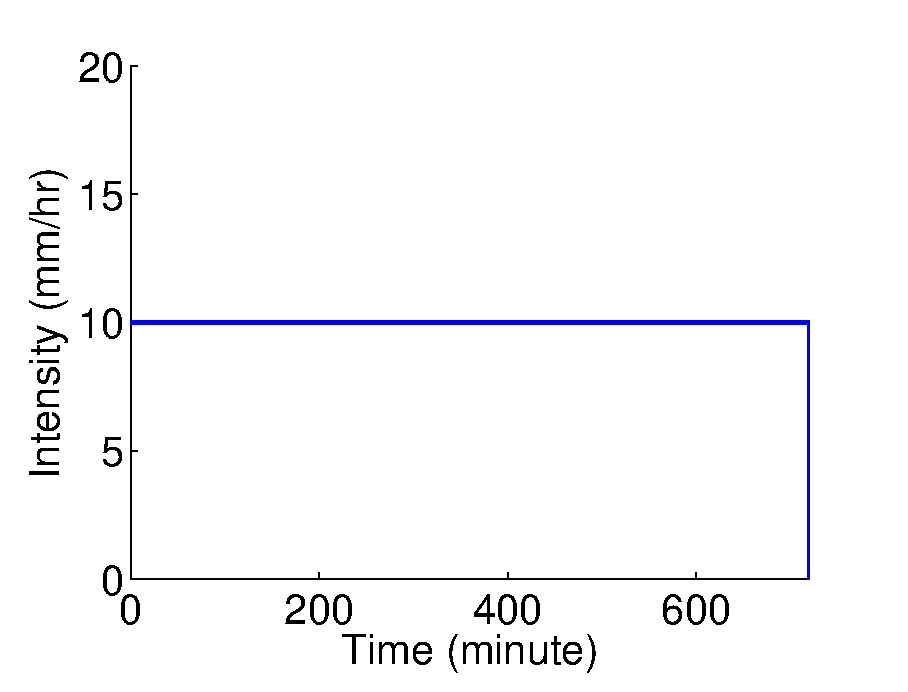
\includegraphics[width=0.24\textwidth]{./img/wepp_input_constant_6hr}}
  \subfloat[]{%
  \label{fig:weppinputincreasedecrease6hr}
  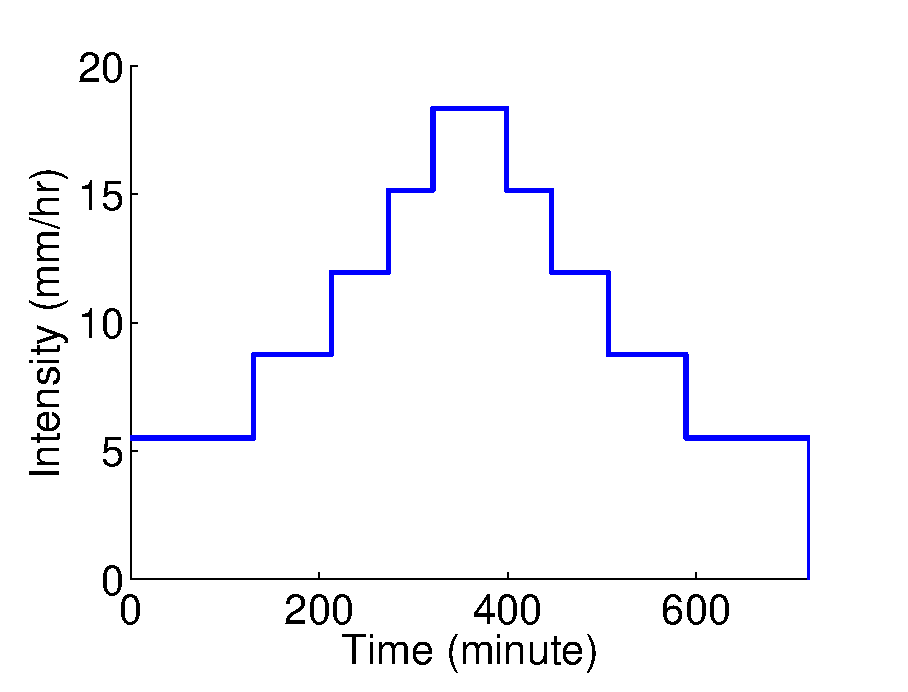
\includegraphics[width=0.24\textwidth]
{./img/wepp_input_increase_decrease_6hr}}
  \caption[Intensity patterns of a stratiform storm for WEPP and EUROSEM
simulations.]{Intensity patterns of a stratiform storm for WEPP and EUROSEM
simulations. All the inputs have the same total rainfall amount (120 mm) and
duration (12 hour). Note the scales of the axes.}
  \label{fig:weppeurosemintensityinputstwelvehours}
\end{figure}

\begin{figure}[htbp]
  \centering
  \subfloat[]{%
  \label{fig:weppinputincrease2hr}
  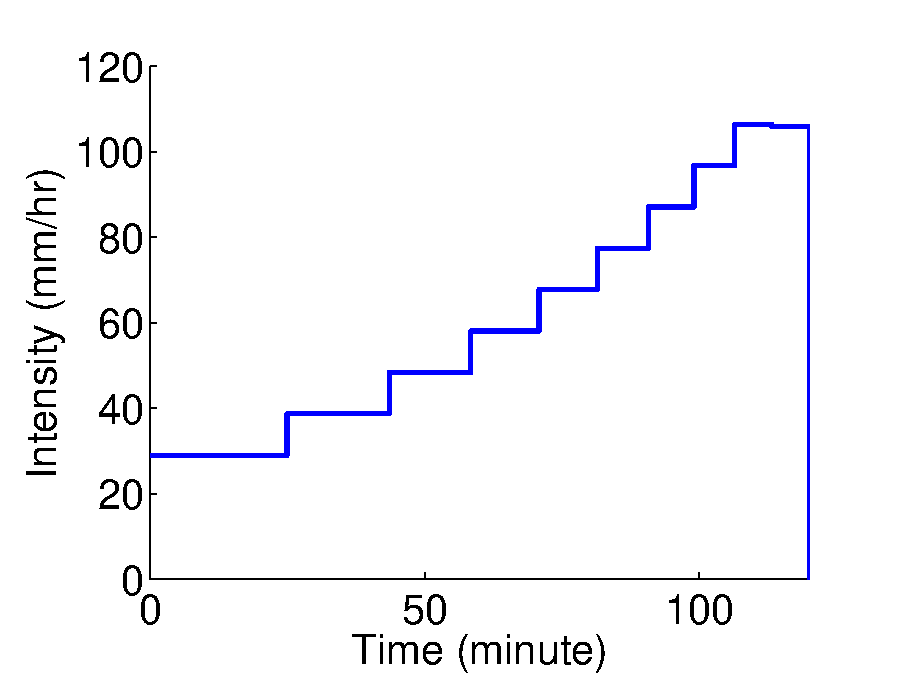
\includegraphics[width=0.24\textwidth]{./img/wepp_input_increase_2hr}}
  \subfloat[]{%
  \label{fig:weppinputdecrease2hr}
  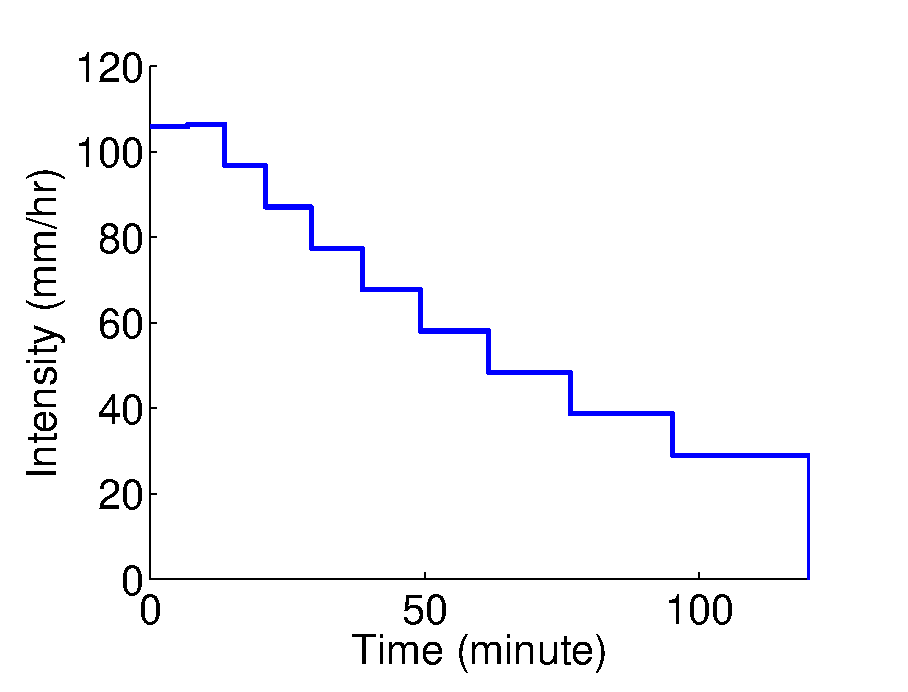
\includegraphics[width=0.24\textwidth]{./img/wepp_input_decrease_2hr}}
  \subfloat[]{%
  \label{fig:weppinputcontrol2hr}
  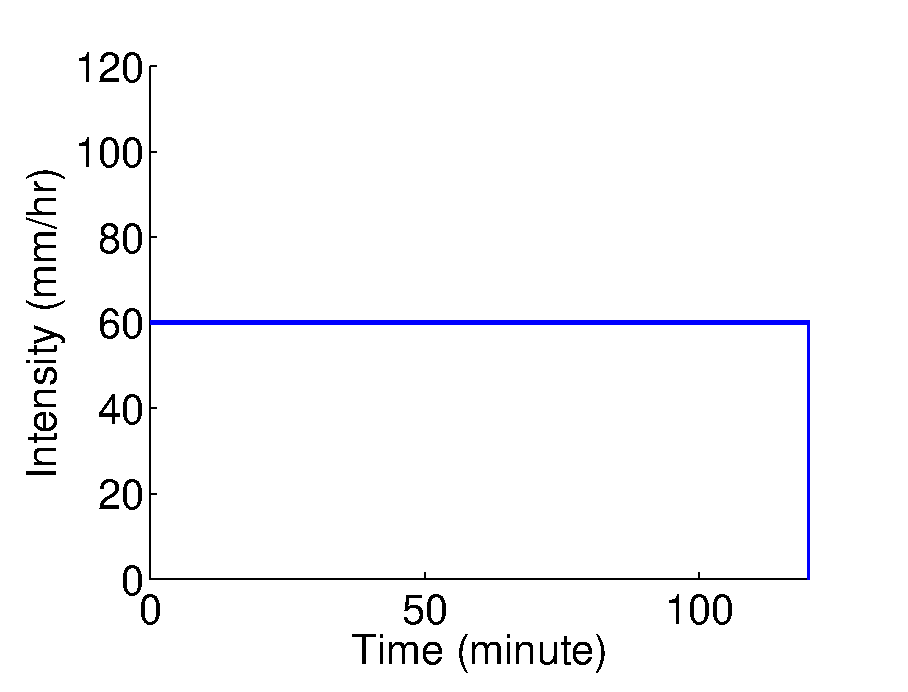
\includegraphics[width=0.24\textwidth]{./img/wepp_input_constant_2hr}}
  \subfloat[]{%
  \label{fig:weppinputincreasedecrease2hr}
  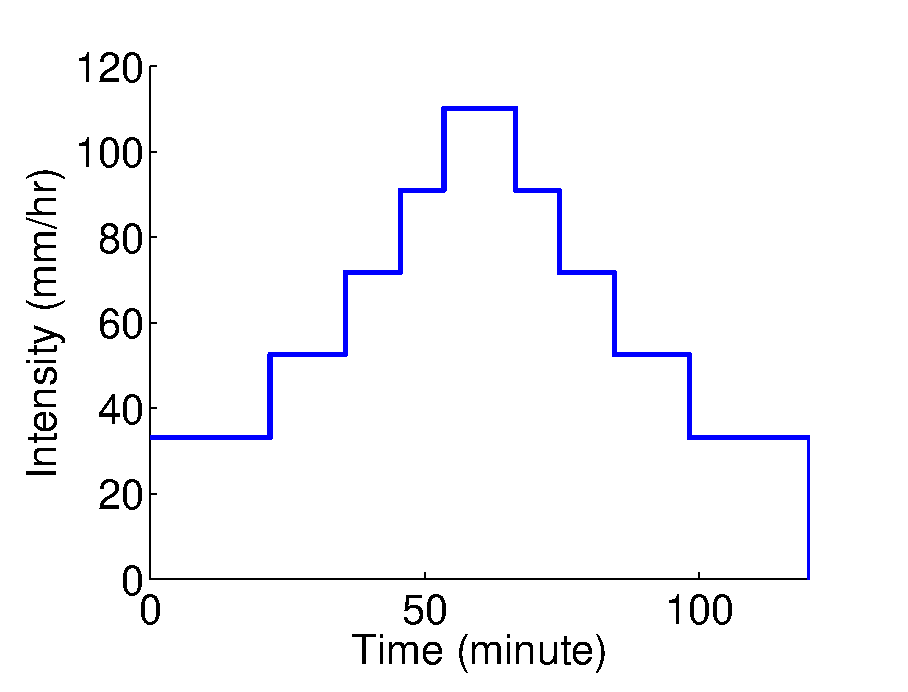
\includegraphics[width=0.24\textwidth]
{./img/wepp_input_increase_decrease_2hr}}
  \caption[Intensity patterns of a convective storm for WEPP and EUROSEM
simulations.]{Intensity patterns of a convective storm for WEPP and EUROSEM
simulations. All the inputs have the same total rainfall amount (120 mm) and
duration (2 hour). Note the scales of the axes.}
  \label{fig:weppeurosemintensityinputstwohours}
\end{figure}

A separate storm with average rainfall intensity of 120 mm/hr (60 mm for 30
min) is designed for RillGrow simulations as shown in Figure
\ref{fig:rillgrow2intensityinputs}. A separate designed storm is used because
of the long computation time required with the version of RillGrow, which is
version 2, as discussed previously. The main aim of this chapter is to
investigate effects of WSIP on erosion modelling. Thus, in principle, using a
separate storm for RillGrow should not have any effects on the investigation
result---this is more discussed later in this chapter.

\begin{figure}[htbp]
  \centering
  \subfloat[]{%
  \label{fig:rg2inputincrease}
  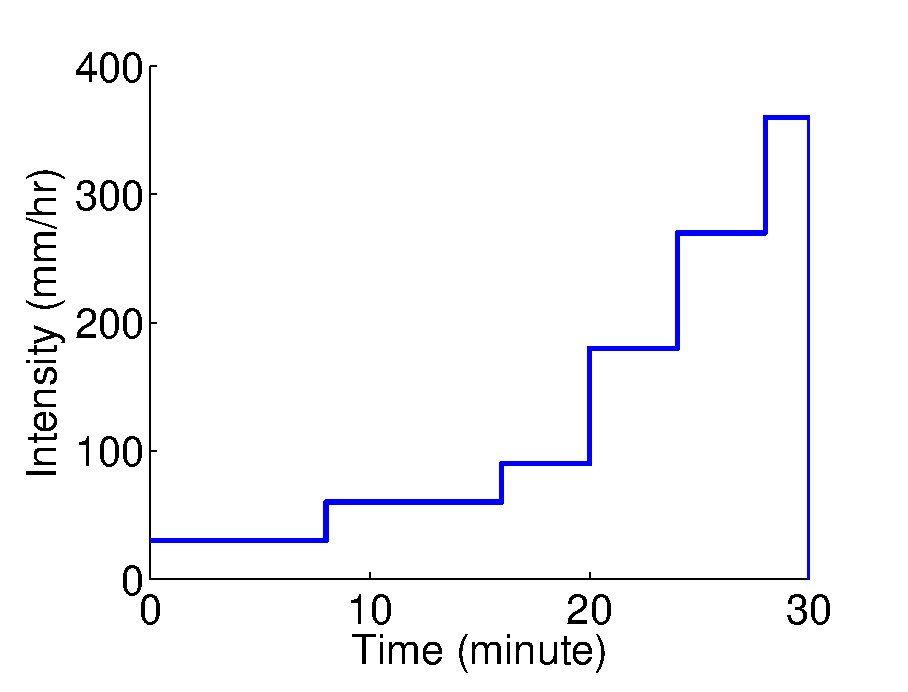
\includegraphics[width=0.24\textwidth]{./img/rg2_input_increase}}
  \subfloat[]{%
  \label{fig:rg2inputdecrease}
  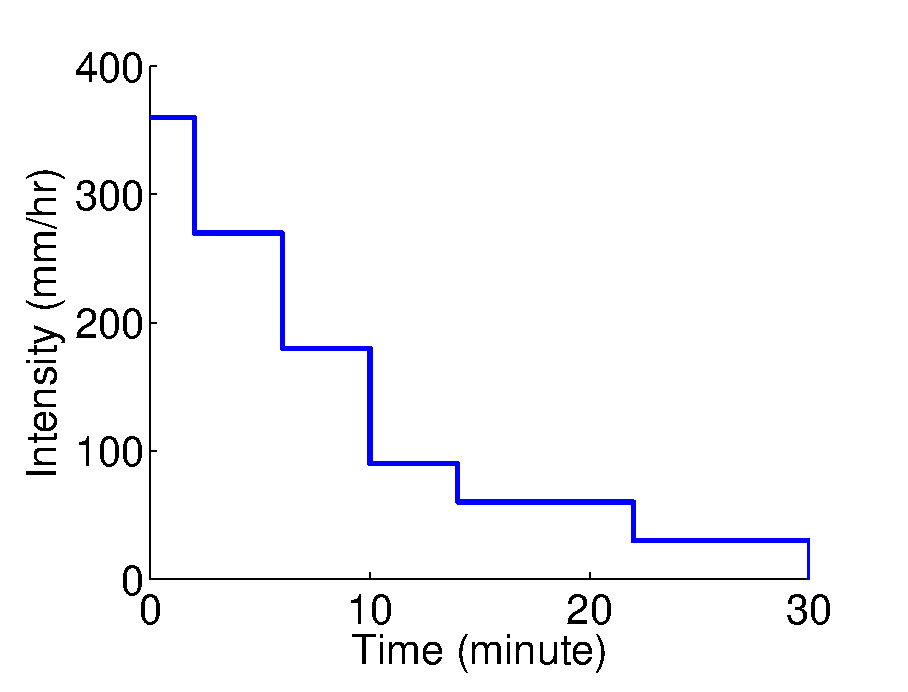
\includegraphics[width=0.24\textwidth]{./img/rg2_input_decrease}}
  \subfloat[]{%
  \label{fig:rg2inputcontrol}
  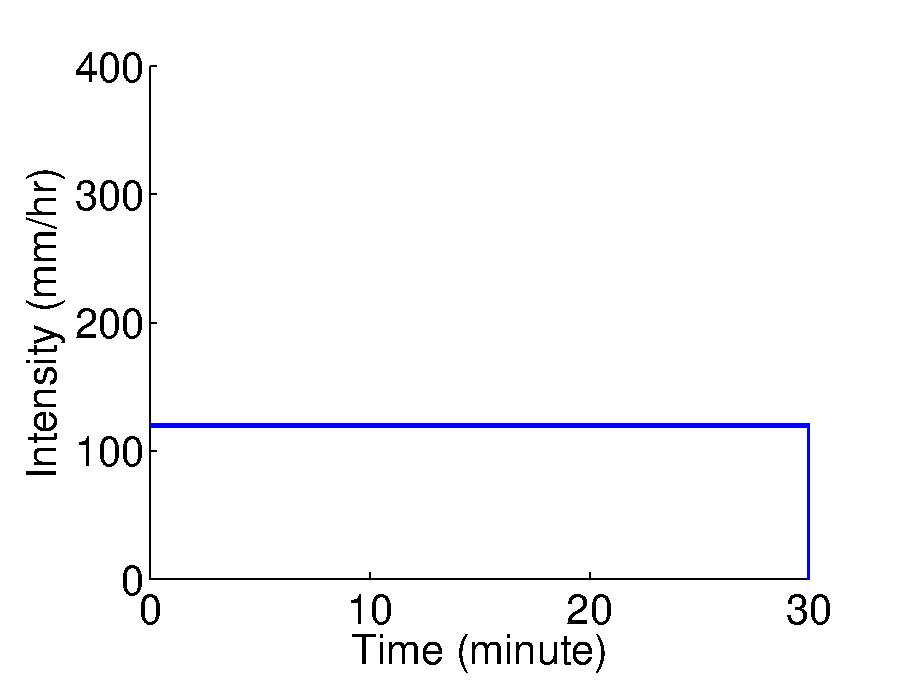
\includegraphics[width=0.24\textwidth]{./img/rg2_input_control}}
  \subfloat[]{%
  \label{fig:rg2inputincreasedecrease}
  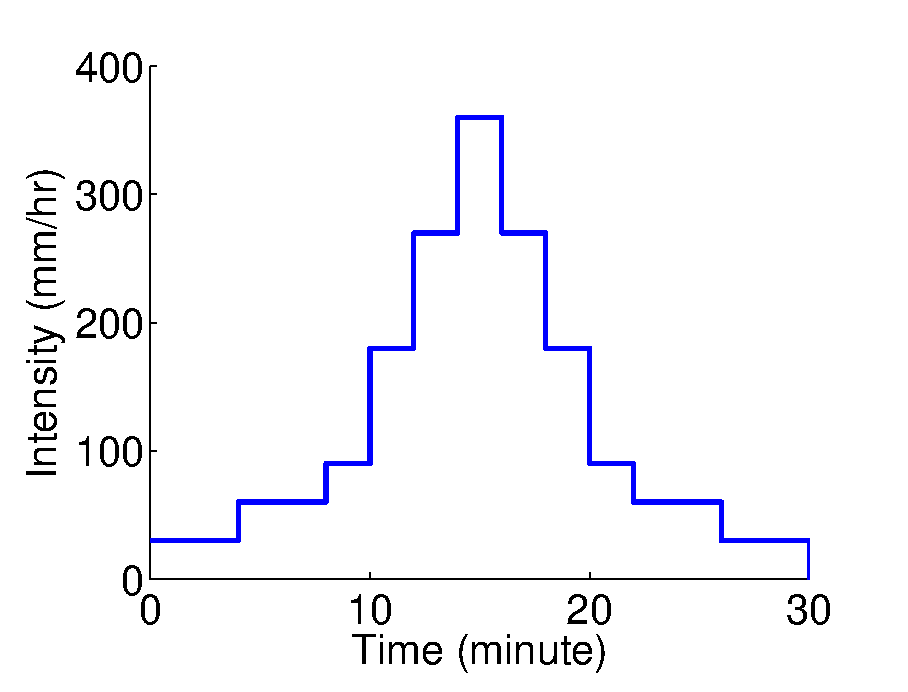
\includegraphics[width=0.24\textwidth]
{./img/rg2_input_increase_decrease}}
  \caption[Intensity input patterns for RillGrow2 simulations.]{Intensity
input patterns for RillGrow2 simulations. All the inputs have the same total
rainfall amount and duration (i.e.\ 60 mm rainfall for 30 minutes). Note the
scales of the axes.}
  \label{fig:rillgrow2intensityinputs}
\end{figure}

The effects of WSIP changes on runoff and soil loss estimated by WEPP, EUROSEM
and RillGrow are shown in the next section.

\section{Effects of WSIPs on Runoff and Soil Loss}
\label{sec:ImplicationsOfRainfallIntensityChangesOnRunoffandSoilLoss}

The summary of WEPP simulation results is shown in Table
\ref{tab:WEPPSimulationResults}. The results are compared against the constant
intensity storm in terms of \% changes. When 60 mm/hr intensity is used, WEPP
estimates the same runoff with all WSIPs. However, for the same intensity, WEPP
estimates soil losses with about 5--9\% increases with increasing, decreasing
and increasing-decreasing WSIPs in comparison to those with the constant WSIP.
In contrast, when lower intensity (i.e.\ 10 mm/hr) is used, WEPP simulates
notably different results. While estimated runoff rates are almost the
same---less than 2\% changes---for all WSIPs, estimated soil loss rates are
increased extensively by 5250\%, 3750\% and 5600\% for increasing, decreasing
and increasing-decreasing WSIPs respectively from the soil loss rate for the
constant WSIP (Table \ref{tab:WEPPSimulationResults}). This is because
WEPP-estimated soil loss rate with the constant intensity pattern is
dramatically small (0.4 t/ha). Runoff and soil loss rates estimated with 60
mm/hr intensity are generally lager than those with 10 mm/hr intensity
regardless of WSIPs.

\begin{table}[htbp]
  \figureversion{tabular}
  \caption{Summary of WEPP simulation results for varying WSIPs}
  \label{tab:WEPPSimulationResults}
  \centering
    \begin{tabular}{lcccc}
      \toprule
      Storm Pattern & \multicolumn{2}{c}{\textbf{60 mm/hr}} &
\multicolumn{2}{c}{\textbf{10 mm/hr}}\\
      \cmidrule(r){2-3} \cmidrule(l){4-5}
      & runoff  & soil loss  & runoff & soil loss\\
      & (mm) & (t/ha) & (mm) & (t/ha)\\
      \midrule
      Constant & 104.2 & 105 & 68.9 & 0.4\\
      Increasing & 104.2 & 114.6 ($+$9.1) & 70.3 ($+$2.0) & 21.4 ($+$5250)\\
      Decreasing & 104.2 & 110.4 ($+$5.1) & 68.6 ($-$0.4) & 15.4 ($+$3750)\\
      Increasing-decreasing & 104.2 & 114.7 ($+$9.2) & 69.9 ($+$1.5) & 22.8
($+$5600)\\
      \bottomrule
      %\addlinespace[1mm]
      \multicolumn{5}{p{10cm}}{\footnotesize Figures in (\ )
are the \% changes from the result with a constant intensity storm. $+/-$
indicates a increase or decrease.}\\
    \end{tabular}
\end{table}

% \begin{sidewaystable}[htbp]
%   \figureversion{tabular}
%   \caption{WEPP simulation results}
%   \label{tab:WEPPSimulationResults}
%   \centering
%     \begin{tabular}{lcccccc}
%       \toprule
%       Storm Pattern & \multicolumn{2}{c}{\textbf{60 mm/hr}} &
% \multicolumn{2}{c}{\textbf{10 mm/hr}} & \multicolumn{2}{c}{\textbf{Mean}}\\
%       \cmidrule(r){2-3} \cmidrule(l){4-5} \cmidrule(l){6-7}
%       & runoff  & soil loss  & runoff & soil loss & runoff &
% soil loss \\
%       & (mm) & (t/ha) & (mm) & (t/ha)& (mm) & (t/ha) \\
%       \midrule
%       Constant & 104.2 & 105 & 68.9 & 0.4 & 86.6 & 52.7 \\
%       Increasing & 104.2 & 114.6 ($+$9.1) & 70.3 ($+$2.0) &
% 21.4 ($+$5250) & 87.3 ($+$0.8) & 68 ($+$29)\\
%       Decreasing & 104.2 & 110.4 ($+$5.1) & 68.6 ($-$0.4)&
% 15.4 ($+$3750) & 86.4 ($-$0.2) & 62.9 ($+$19.4)\\
%       Increasing-decreasing & 104.2 & 114.7 ($+$9.2) & 69.9
% ($+$1.5) & 22.8 ($+$5600) & 87.1 ($+$0.6) & 68.8 ($+$30.6)\\
%       \bottomrule
%       %\addlinespace[1mm]
%       \multicolumn{7}{p{15cm}}{\footnotesize Figures in (\ )
% are the \% changes from the result with a constant intensity storm. $+/-$
% indicates a increase or decrease.}\\
%     \end{tabular}
% \end{sidewaystable}

The summary of EUROSEM simulation results is shown in Table
\ref{tab:EUROSEMSimulationResults}. For 60 mm/hr and 10 mm/hr intensity,
EUROSEM shows the similar responses. When runoff rates estimated by EUROSEM with
varying WSIPs with 60 mm/hr and 10 mm/hr intensities are compared to those
estimated with the constant WSIP for both intensities, there are not much
differences in estimated runoff rates. The magnitude of changes are around
0.3--3\% although runoff estimated with 10 mm/hr intensity is smaller than
runoff estimated with 60 mm/hr intensity. On the other hand, there are slight
decreases in estimated soil loss rates with increasing, decreasing and
increasing-decreasing WSIPs in comparison to those estimated with the constant
WSIP. Unlike WEPP results, soil loss results show decreases, which are in the
similar magnitude, for both intensities: 60 mm/hr and 10 mm/hr. Constant WSIP
simulates the largest soil loss rates: 22.6 t/ha and 24.7 t/ha for 60 mm/hr and
10 mm/hr, respectively. The smallest soil loss rates are estimated with
increasing WSIP: 19.7 t/ha and 22.1 h/ha for 60 mm/hr and 10 mm/hr, respectively
(Table \ref{tab:EUROSEMSimulationResults}).

\begin{table}[htbp]
  \figureversion{tabular}
  \caption{Summary of EUROSEM simulation results for varying WSIPs}
  \label{tab:EUROSEMSimulationResults}
  \centering
    \begin{tabular}{lcccc}
      \toprule
      Storm Pattern & \multicolumn{2}{c}{\textbf{60 mm/hr}} &
\multicolumn{2}{c}{\textbf{10 mm/hr}}\\
      \cmidrule(r){2-3} \cmidrule(l){4-5}
      & runoff  & soil loss  & runoff & soil loss \\
      & (mm) & (t/ha) & (mm) & (t/ha) \\
      \midrule
      Constant   & 101.4 & 22.6 & 73.8 & 24.7\\
      Increasing & 98.7 ($-$2.7)& 19.7 ($-$12.8)& 75.5 ($+$2.3)& 22.1
($-$10.5)\\
      Decreasing & 103.5 ($+$2.1)& 22.2 ($-$1.8)& 74.0 ($+$0.3) & 24.1
($-$2.4)\\
      Increasing-decreasing & 103.3 ($+$1.9)& 21.0 ($-$7.1)& 76.0 ($+$3.0)& 22.7
($-$8.1)\\
      \bottomrule
      %\addlinespace[1mm]
      \multicolumn{5}{p{10cm}}{\footnotesize Figures in (\ )
are the \% changes from the result with a constant intensity storm. $+/-$
indicates a increase or decrease.}\\
    \end{tabular}
\end{table}

% \begin{sidewaystable}[htbp]
%   \figureversion{tabular}
%   \caption{EUROSEM simulation results}
%   \label{tab:EUROSEMimulationResults}
%   \centering
%     \begin{tabular}{lcccccc}
%       \toprule
%       Storm Pattern & \multicolumn{2}{c}{\textbf{60 mm/hr}} &
% \multicolumn{2}{c}{\textbf{10 mm/hr}} & \multicolumn{2}{c}{\textbf{Mean}}\\
%       \cmidrule(r){2-3} \cmidrule(l){4-5} \cmidrule(l){6-7}
%       & runoff  & soil loss  & runoff & soil loss & runoff &
% soil loss \\
%       & (mm) & (t/ha) & (mm) & (t/ha)& (mm) & (t/ha) \\
%       \midrule
%       Constant   & 101.4 & 22.6 & 73.8 & 24.7 & 87.6 & 23.7 \\
%       Increasing & 98.7 ($-$2.7)& 19.7 ($-$12.8)& 75.5
% ($+$2.3)& 22.1 ($-$10.5)& 87.1 ($-$0.6)& 21.0 ($-$11.4)\\
%       Decreasing & 103.5 ($+$2.1)& 22.2 ($-$1.8)& 74.0 ($+$0.3) & 24.1 ($-$2.4)&
% 88.8 ($+$1.4)& 23.2 ($-$2.1)\\
%       Increasing-decreasing & 103.3 ($+$1.9)& 21.0 ($-$7.1)&
% 76.0 ($+$3.0)& 22.7 ($-$8.1)& 89.7 ($+$2.4)& 21.9 ($-$7.6)\\
%       \bottomrule
%       %\addlinespace[1mm]
%       \multicolumn{7}{p{15cm}}{\footnotesize Figures in (\ )
% are the \% changes from the result with a constant intensity storm. $+/-$
% indicates a increase or decrease.}\\
%     \end{tabular}
% \end{sidewaystable}

The summary of RillGrow simulation results is shown in Table
\ref{tab:RillGrowSimulationResults}. Again, runoff, which is simulated as
``Totals lost from edges (litre)'', for increasing, decreasing and
increasing-decreasing WSIPs does not show much changes from that of the constant
WSIP. However, estimated soil loss rates changes when the different WSIPs are
used. The largest soil loss rate (90.5 t/ha) is estimated with decreasing WSIP
while the constant WSIP produces the smallest soil loss rate (64 t/ha) (Table
\ref{tab:RillGrowSimulationResults}). Similar to WEPP results, increasing,
decreasing and increasing-decreasing WSIPs result in increases (about 15--40\%)
in soil loss rates in comparison to the soil loss rates estimated with the
constant WSIP.

\begin{table}[htbp]
  \figureversion{tabular}
  \centering
  \small
  \caption{Summary of RillGrow simulation results for varying WSIPs}
  \label{tab:RillGrowSimulationResults}
    \begin{tabular}{lcc}
    \toprule
     & Totals lost from edges$^\dagger$ (litre) & Soil Loss (t/ha)\\
    \midrule%
    Constant & 471.9 & 64.0 \\
    Increasing & 472.4 ($+$0.1)& 73.5 ($+$14.8)\\
    Decreasing & 471.2 ($-$0.2)& 90.5 ($+$41.4)\\
    Increasing-decreasing & 472.2 ($+$0.1)& 82.6 ($+$29.1)\\
    \bottomrule
    %\addlinespace[1mm]
    \multicolumn{3}{p{11cm}}{\footnotesize $^\dagger$ No
infiltration was considered. Every rain runs off the edge of the simulated plot.
Figures in (\ ) are the \% changes from the result with a constant intensity
storm. $+/-$ indicates a increase or decrease.}\\
    \end{tabular}
\end{table}

%Discuss how the models respond to each rainfall patterns. Which one
%produced most runoff and soil loss?
%Which on produced least runoff and soil loss?

%What's the potential problem with constant intensity generating least
%runoff and soil loss (WEPP)?
%GCM and RCM data scale. knowing average daily rainfall intensity is not
%sufficient for erosion estimation. It may lead to underestimated erosion
%with low average intensity rainfall.

\section{Discussion}
\label{sec:ImpactsOfRainfallIntensityChangesOnRunoffAndErosionDiscussion}

\paragraph{Effect of WSIP on WEPP result} In WEPP inputs, $t_p$ represents
normalised time-to-peak which is closely related to WSIP. This parameter, $t_p$,
was previously considered not much sensitive \citep{nearing1990-839}.
\citet{nearing1990-839} performed sensitivity analysis on WEPP, which was
still in the early stage of its development, by assessing various input
variables such as soil, plant residue and canopy, hillslope topography, and
hydrologic input variables. They calculated sensitivity parameter, $S$, as a
relative normalised change in output to a normalised change in input.
They concluded that \emph{peak rainfall intensity}, \emph{time to peak rainfall
intensity}, rill spacing and width, and sediment transportability were not
playing a major role in soil loss predictions.

Their findings may not be compared directly with the result presented in this
chapter because their analysis was carried out on the developing version of WEPP
while this chapter used more recent version of WEPP and the intensity value they
used was much higher (100 mm/hr) than the intensities (10 and 60 mm/hr) used in
this chapter.

However, as seen in Table \ref{tab:WEPPSimulationResults}, the timing of peak
intensity (or WSIP in this chapter), had visible effects on the result of
simulations. It became even more evident when rainfall with low intensity (10
mm/hr) was used with WEPP. For example, when the constant WSIP was used for WEPP
simulations, WEPP greatly underestimated soil loss rates by about 50 times less
than the average soil loss rate of other WISPs---increasing, decreasing and
increasing-decreasing WSIPs (Table \ref{tab:WEPPSimulationResults}). Thus, it is
essential to know about WSIP of the rainfall storm that is used for erosion
simulations.

The difference in soil loss with this magnitude (i.e.\ 50 times) is worryingly
large and raises considerable problems, for example, when GCM/RCM rainfall data
are directly used for soil erosion modelling. This is because GCM/RCM data are
usually used as daily data in which no peak intensity can be identified. In
other words, they are used as constant WSIP. Moreover, as discussed previously,
disaggregation of such data into sub-daily data is not viable as it increases
uncertainty in erosion estimation results.

\paragraph{Effect of WSIP on EUROSEM result} EUROSEM, however, resulted in
rather different results from WEPP simulation results. Although EUROSEM
estimation results were also affected by the change of WSIP, unlike WEPP,
EUROSEM simulated less soil loss with increasing, decreasing and
increasing-decreasing WSIPs than that with constant WSIP (Table
\ref{tab:EUROSEMSimulationResults}). In fact, soil loss rates estimated with
increasing WSIP was the smallest soil loss rate.

Detailed investigations of the EUROSEM output files showed that slightly less
``Gross Interrill Erosion'' was estimated with increasing WSIP than with other
WSIPs while ``Gross Rill Erosion'' was estimated at the similar rate for all
WSIPs. This was however only seen with 60 mm/hr intensity. When 10 mm/hr
intensity was used, EUROSEM estimated slightly less ``Gross Rill Erosion'' with
increasing WSIP than with other WSIPs. ``Gross Interrill Erosion'' was almost
negligible for all four WSIPs when 10 mm/hr intensity was used. This confirms
again that EUROSEM dynamically changes its modelling mode depending on the
surface condition so that the proportion of rill and interrill erosion for the
total erosion changes. Also, This shows that the responses of EUROSEM---in
terms of total erosion rates---to the change of WSIP are the same regardless of
the average rainfall intensity: the smallest soil loss rate is estimated with
increasing WSIP.

In addition, in comparison to the previous chapter, Chapter
\ref{sec:EFFECTSOFCONTINOUSANDDISCONTINUSSTORM}, EUROSEM estimated increased
soil loss with lower average intensity (10 mm/hr) than with higher average
intensity (60 mm/hr). This increase of soil loss rates was even accompanied with
decreased runoff rates. These EUROSEM simulation results are unrealistic and may
imply that EUROSEM is subject to some model improvements in this regard.

\paragraph{Effect of WSIP on RillGrow result} RillGrow simulated, for constant
WSIP, about 78\% soil loss from the average soil loss of storms with other
WSIPs. RillGrow also estimated the largest soil loss with decreasing WSIP in
comparison to those estimated with other storm patterns. Runoff simulated by
RillGrow with varying WSIPs was, on the other hand, not affected because of no
infiltration was considered as discussed in the previous chapter.

The result from RillGrow simulations with constant and decreasing WSIPs was
consistent with the result from the study by \citet{parsons2006-68}.
\citet{parsons2006-68} conducted a series of lab experiments to investigate the
effects of five different intensity patterns (i.e.\ constant, increasing,
decreasing, increasing then decreasing and decreasing then increasing intensity)
on soil erosion (Table \ref{tab:Tonysexperimentresults}). They found that the
constant-intensity storm generated the least amount of soil loss which was about
75\% of the average soil loss for the variable-intensity storms. Also, the
largest soil loss amount was occurred when decreasing-intensity pattern was
used.

\begin{table}[htbp]
  \figureversion{tabular}
  \caption[Experiment results]{Experiment results
\citep[From][]{parsons2006-68}}
  \label{tab:Tonysexperimentresults}
  \scriptsize
  \centering
    \begin{tabular}{lcccccccccc}
      \toprule
      Storm Pattern & \multicolumn{2}{c}{Clay loam} &
\multicolumn{2}{c}{\textbf{Sandy loam}} & \multicolumn{2}{c}{Sandy soil} &
\multicolumn{2}{c}{\textbf{Total}}\\
      \cmidrule(r){2-3} \cmidrule(rl){4-5} \cmidrule(rl){6-7}
\cmidrule(l){8-9}
      & runoff (l) & loss (g) & runoff (l) & loss (g) & runoff
(l) & loss (g) & runoff (l) & loss (g)\\
      \midrule
      Constant & 131.6 & 523 & 83.4  & 1256 & 110.2 & 2509 &
325.2 & 4289\\
      Increasing & 108.2 & 748 & 93.0  & 2435 & 72.2 & 1947 &
273.4 & 5130 \\
      Decreasing & 101.3 & 456 & 114.0 & 3230 & 108.3 & 2862 &
323.6 & 6548 \\
      Rising-falling & 110.4 & 631 & 95.8  & 2110 & 114.2 &
3584 & 320.4 & 6324\\
      Falling-rising$^\dagger$ & 103.6 & 629 & 103.9  & 1645 &
108.1 & 3275 & 315.6 & 5549\\
      \bottomrule
      %\addlinespace[1mm]
      \multicolumn{9}{p{11cm}}{\footnotesize $^\dagger$ Not
used in this research since only one peak intensity is assumed for all model
simulations.}\\
    \end{tabular}
\end{table}

By comparing the soil loss results estimated with WEPP, EUROSEM and RillGrow
with the result from \citet{parsons2006-68}, it was found that RillGrow showed
the similar results for constant and decreasing WSIPs with which the smallest
and largest soil loss rates were simulated, respectively (Table
\ref{tab:MagnitudeofSoilLossAffectedByIntraStormPatterns}). Also, WEPP showed
the consistent results with \citet{parsons2006-68} for constant and increasing
WSIPs with which the smallest and the second largest soil loss rates were
estimated, respectively. However, some of other simulation results were not
consistent with the result from \citet{parsons2006-68}. For example, EUROSEM
simulation results were completely inconsistent as the largest soil loss was
estimated by EUROSEM with constant WSIP and the smallest soil loss was
estimated with increasing WSIP.

\begin{table}[htbp]
  \centering
  \scriptsize
  \caption{Magnitude of soil loss affected by WSIPs}
  \label{tab:MagnitudeofSoilLossAffectedByIntraStormPatterns}
    \begin{tabular}{cllll}
      \toprule
      Soil Loss & \citet{parsons2006-68}  & WEPP & EUROSEM &
RillGrow \\
                & (Sandy loam) & (Mean) & (Mean) & \\
      \midrule
      High & decreasing & increasing-decreasing & constant &
decreasing\\
      $\Uparrow$ & increasing & increasing & decreasing &
increasing-decreasing\\
      $\Downarrow$ & increasing-decreasing & decreasing &
increasing-decreasing & increasing\\
      Low & constant & constant & increasing & constant\\
      \bottomrule
    \end{tabular}
\end{table}

Despite WEPP and RillGrow simulation results were partially consistent with the
results from \citet{parsons2006-68}, they still showed inconsistent responses to
the change of WSIP for, for example, WEPP with increasing-decreasing and
decreasing WSIPs and RillGrow with increasing-decreasing and increasing WSIPs.
This means that erosion models still simulate different responses to the change
of WSIP compared to the measured responses. This difference need to be improved
by more lab or field experiments that can be compared to the model results.
As fas as this research is aware, there are no other lab or field experiments
that can be compared against model responses to the change of WSIPs except the
study by \citet{parsons2006-68}. Thus, there is an urgent need for such
research.

\section{Conclusion}
\label{sec:ImpactsOfRainfallIntensityChangesOnRunoffAndErosionConclusion}
It was shown in this chapter that WSIP (or $t_p$ for WEPP) is a important factor
for erosion estimations. Without knowing details of WSIPs, erosion models could
easily estimate soil erosion with great variabilities as shown in WEPP results.
Effects of WSIPs on runoff estimations were however small implying WSIP
affects soil loss rate more.

The change of WSIP with high intensity have less impacts on soil loss
estimations than the change of WSIP with low intensity. Despite varying
responses of the erosion models to the change of WSIP, constant WSIP produced
the least soil loss when used with WEPP and RillGrow.

There are urgent needs for more lab or field experiments that can be compared
with the model results in order to improve model predictabilities.

%\nolinenumbers

\section{Summary of Model Simulation Result: Effect of WSIV, WSG and WSIP}
\label{sec:SummaryOftheSimulationResults}

%More can be learned from difficulties encountered \citep{jetten1999-521}.

In Part \ref{sec:RAINFALLINTENSITYCHANGESANDSOILEROSION}, \textit{Rainfall
Intensity and Erosion: Model Descriptions and Responses}, various factors, which
are related to rainfall intensity of a storm, have been investigated in
terms of their effects on soil erosion. These factors (i.e.\ temporal
resolution of rainfall data, WSG and WSIP) are closely related to the
simulation result that are estimated by WEPP, EUROSEM and RillGrow.

During these investigations, we have found:
\begin{itemize}
  \item Chapter \ref{sec:EFFECTSOFTEMPORALSCALESOFSTROMDATA}:
  \begin{itemize}
      \item Temporal resolutions of rainfall data affect Within-Storm Intensity
Variations (WSIVs)
      \item Temporal resolutions of rainfall data are closely related to the
estimated results of runoff and soil loss
      \item In terms of soil loss, WEPP is more sensitive to the change of
temporal data resolutions than EUROSEM
      \item Erosion estimations with CLIGEN data are more affected by the change
of temporal resolutions than those with breakpoint data
      \item Breakpoint data are preferred to CLIGEN data as far as
investigations on effects of rainfall intensity on erosion are concerned
      \item For the subsequent analyses of this research, 15-min breakpoint
rainfall data are chosen
  \end{itemize}
  \item Chapter \ref{sec:EFFECTSOFCONTINOUSANDDISCONTINUSSTORM}:
    \begin{itemize}
      \item Within-Storm Gaps (WSGs) affected estimated runoff and soil loss by
WEPP and EUROSEM.
      \item WSG have almost no effect on runoff and soil loss estimated by
RillGrow.
      \item Although it was not evident to conclude whether WSGs have
positive or negative effects on runoff and soil loss estimations, the removal
of WSGs from original data affected model simulation results.
      \item Thus, removing WSGs from the original rainfall data is not
recommended
      \item Analyses of outputs from WEPP simulations revealed new problem
that WEPP modifies original rainfall intensity and simulates unrealistic
results.
      \item When breakpoint data with temporal resolutions shorter than
60-min temporal resolution is used for WEPP simulations, WEPP constructs
``WEPP-modified'' rainfall data which have different rainfall intensity
information from original rainfall intensity.
    \end{itemize}
  \item Chapter \ref{sec:EFFECTSOFRAINFALLINTENSITYCHANGESONSOILEROSION}:
    \begin{itemize}
      \item Within-Storm Intensity Pattern (WSIP) affects soil loss rates
estimated by WEPP, EUROSEM and RillGrow.
      \item Effects of the change of WSIP on runoff rates estimated by the same
models are relatively small compared to those on estimated soil loss rates.
      \item The change of WSIP with high intensity have less impacts on soil
erosion estimations than the change of WSIP with low intensity.
      \item The smallest soil loss rate was estimated with constant WSIP when
WEPP and RillGrow were used
      \item Comparisons with the result from the only laboratory experiment by
\citet{parsons2006-68} showed that WEPP and RillGrow simulation results are
almost consistent to the observational result: The smallest soil loss rate was
estimated by WEPP and RillGrow with constant WSIP.
    \end{itemize}
\end{itemize}

The effect of intensity-related factors on runoff and soil loss found in Part
\ref{sec:RAINFALLINTENSITYCHANGESANDSOILEROSION} are summarised in Table
\ref{tab:SimulationSummary}.

\begin{sidewaystable}[htbp]
% \small
  \centering
  \caption{Summary of the effect of within-storm intensity characteristics on
runoff and soil erosion}
  \label{tab:SimulationSummary}
    \begin{tabular}{llcccc}
    \toprule
    & & \multicolumn{3}{c}{Erosion Model} & Measurement \\
    \cmidrule(rl){3-5} \cmidrule(rl){6-6}
    Intensity Pattern & & WEPP$^1$ & EUROSEM$^1$ & RillGrow &
\citet{parsons2006-68}$^2$\\
    \midrule
    \midrule
    Constant & Runoff & $-$ & $-$ & $-$ & $-$ \\
             & Soil loss & $-$ & $-$ & $-$ & $-$ \\
    \midrule
    Increasing$^\dagger$ & Runoff & $-$ & $-$ & $-$ &
$\blacktriangle\blacktriangle$ \\
                         & Soil loss &
$\blacktriangle\blacktriangle\blacktriangle$ & $\triangledown\triangledown$
& $\blacktriangle\blacktriangle$ &
$\blacktriangle\blacktriangle\blacktriangle\blacktriangle\blacktriangle$ \\
    \midrule
    Decreasing$^\dagger$ & Runoff & $-$ & $\triangledown$ & $-$ &
$\blacktriangle\blacktriangle\blacktriangle\blacktriangle$\\
                         & Soil loss &
$\blacktriangle\blacktriangle\blacktriangle$ & $\triangledown$ &
$\blacktriangle\blacktriangle\blacktriangle\blacktriangle$ &
$\blacktriangle\blacktriangle\blacktriangle\blacktriangle\blacktriangle$ \\
    \midrule
    Increasing-Decreasing$^\dagger$ & Runoff & $-$ & $\triangledown$ & $-$ &
$\blacktriangle\blacktriangle$ \\
                                    & Soil loss &
$\blacktriangle\blacktriangle\blacktriangle\blacktriangle$ &
$\triangledown\triangledown$ & $\blacktriangle\blacktriangle\blacktriangle$
& $\blacktriangle\blacktriangle\blacktriangle\blacktriangle\blacktriangle$ \\
    \midrule
    \midrule
    Continuous & Runoff & $-$ & $-$ & $-$ & n/a \\
               & Soil loss & $-$ & $-$ & $-$ & n/a \\
    \midrule
    Discontinuous$^\ddagger$ & Runoff & $\triangledown\triangledown$ &
$\triangledown\triangledown$ & $-$ & n/a \\
                             & Soil loss & $\blacktriangle$&
$\triangledown\triangledown$ & $-$ & n/a\\
    \bottomrule
    %\addlinespace[1mm]
    \multicolumn{6}{p{16cm}}{\scriptsize
    $^1$ Mean runoff and soil loss rate at the average intensity of 60 mm/hr and
10 mm/hr;
    $^2$ Runoff and soil loss rate for Constant Intensity was measured on a
experiment plot filled with sandy loam at an average intensity of 93.9 mm/hr;
    $^\dagger$ Magnitude of changes in comparison with Constant Intensity;
    $^\ddagger$ Magnitude of changes in comparison with Continuous Intensity;
    $-$: unchanged or $\geq$1\% changed;
    $\blacktriangle$: 1$<\Delta\geq$5\% increase;
    $\blacktriangle\blacktriangle$: 5$<\Delta\geq$15\% increase;
    $\blacktriangle\blacktriangle\blacktriangle$: 15$<\Delta\geq$30\%
increase;
    $\blacktriangle\blacktriangle\blacktriangle\blacktriangle$:
30$<\Delta\geq$40\% increase;

$\blacktriangle\blacktriangle\blacktriangle\blacktriangle\blacktriangle$:
$>$40\% increase;
    $\triangledown$: 1$<\Delta\geq$5\% decrease;
    $\triangledown\triangledown$: 5$<\Delta\geq$15\% decrease;
    $\triangledown\triangledown\triangledown$: 15$<\Delta\geq$30\% decrease;
    $\triangledown\triangledown\triangledown\triangledown$:
30$<\Delta\geq$50\% decrease;
    $\triangledown\triangledown\triangledown\triangledown\triangledown$:
$>$40\% decrease}\\
    \end{tabular}
\end{sidewaystable}

Unarguably, there are more studies on effects of rainfall amount on runoff and
soil loss rates than studies on effects of rainfall intensity. This may be
because our interests are given more to the relationship between soil erosion
and rainfall amount than relationship between soil erosion and rainfall
intensity, or maybe because details of rainfall intensity are simply difficult
to record and obtain. In any case, this research showed that the changes of
rainfall intensity play an important role in erosion modelling, and recognised
the need for more researches that looks into the effect of rainfall intensity
changes on runoff and soil loss.

Currently, only observational results available for the comparison analyses were
from the laboratory experiment carried out by \citet{parsons2006-68}. Their
research only concerns about the effect of WSIP changes. However, as shown in
this research, more experiment studies on other intensity-related factors
considered in this thesis such as WSG and WSIV are required. It will then enable
us to understand more on the interaction between rainfall intensity and soil
erosion. Needless to say, without being able to predict (or simulate) present
soil erosion, it will be very hard to accept any prediction done for the future
condition because of possible increases of uncertainty for the future.

The result of this research is however limited by the lack of observational
data. All of the results showed here are model-estimated values and only a small
number of modelling results was compared to the observed (or lab-experimented)
data. This limitation can only be solved by comparing the estimated result
against observational results from more laboratory or field experiments.